\documentclass{article}
\usepackage{graphicx} % new way of doing eps files
\usepackage{listings} % nice code layout
\usepackage[usenames]{color} % color
\definecolor{listinggray}{gray}{0.9}
\definecolor{graphgray}{gray}{0.7}
\definecolor{ans}{rgb}{1,0,0}
\definecolor{blue}{rgb}{0,0,1}
% \Verilog{title}{label}{file}
\newcommand{\Verilog}[3]{
  \lstset{language=Verilog}
  \lstset{backgroundcolor=\color{listinggray},rulecolor=\color{blue}}
  \lstset{linewidth=\textwidth}
  \lstset{commentstyle=\textit, stringstyle=\upshape,showspaces=false}
  \lstset{frame=tb}
  \lstinputlisting[caption={#1},label={#2}]{#3}
}


\author{your names}
\title{Lab title}

\begin{document}
\maketitle

\section{Introduction}
Introduction with problem overview, your design procedure, and rationale.  Be as brief as possible to let me know the big picture of the lab.

\section{Interface}
This section explains the input and output relationships of the design, so it can be treated as a black box.  I have essentially provided you the inputs, outputs, and inouts, but I want to know you understand why.  What inputs are used and how?  What outputs are used and how?  What sequence of commands need to be performed in order to operate the module?  What form does the data get sent in (binary, two's compliment, excess code, etc.)?  How are they grouped?

\section{Design}
This is the internal design of the item.  Design description and explanation, including any pictures, charts, etc.  This is the details of what you want to build, but not how to build it.  In senior design terms, this is the specification.

\section{Implementation}
The Verilog code and explanations of why you implemented this way.  There are many ways to implement a given design in Verilog.  For instance why choose a case statement or ifs?  Why did you trigger on a negedge verses any signal change?  You should reference your code, for example, mine is in Listing~\ref{code:reg} on page~\pageref{code:reg}.  Note you don't have to reference the page, I just wanted to show you how you could, and the power of a label in \LaTeX\ .

\Verilog{Verilog code for implementing a register.}{code:reg}{../code/1_fetch/register.v}

\section{Test Bench Design}
This is where you discuss the test benches you wrote, and what they were designed to test.  You should discuss expected errors as well as random errors.  Be sure to include your Verilog code of the testbench, for example, mine is in Listing~\ref{code:regtest} on page~\pageref{code:regtest}.

\Verilog{Verilog code for testing a register.}{code:regtest}{../code/1_fetch/register_test.v}

\section{Simulation}
In this section you should show the results of your simulation, such as timing diagrams and explain any design issues you had to deal with.  A sample timing diagram is in Figure~\ref{fig:regtest} on page~\pageref{fig:regtest}.

\begin{figure}
\begin{center}
\caption{Timing diagram for the register test.}\label{fig:regtest}
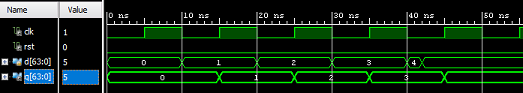
\includegraphics[width=0.9\textwidth]{../images/registertiming.png}
\end{center}
\end{figure}

\section{Conclusions}
Overview the main points you want to stick in peoples minds and answer key questions you want to stick in peoples minds.  Did it work?  How well? What would you have done differently?  What did you learn?
\end{document} 